\chapter{Background}\label{chapter:background}

In modern cryptography one can differ between symmetric and asymmetric encryption schemes. While in a symmetric scheme the decryption and encryption of data is processed with the same key, asymmetric protocols introduce a key pair for every participant: A public key for encryption and a private key for decryption. The public key of asymmetric protocols is, as the name suggests, public to everyone. However, the private key needs to be secret and nobody but the producer may have knowledge about the private key.

\subsubsection{Symmetric Cryptography}

In \autoref{fig:symmetric-encryption} a classical symmetric encryption scheme is shown. First, a plaintext is encryption using a symmetric encryption algorithm and a secret key. The resulting chiffre text is transported to the receiver, where it is decrypted using the appropriate decryption algorithm and the same secret key.  The red section in the middle represents an insecure channel (e.g. the internet), where attackers may read or modify data. A critical question is the exchange of the key through the insecure channel. Somehow the symmetric key needs to be transported securely to the receiver of the chiffre.

\begin{figure}[htpb]
  \centering
  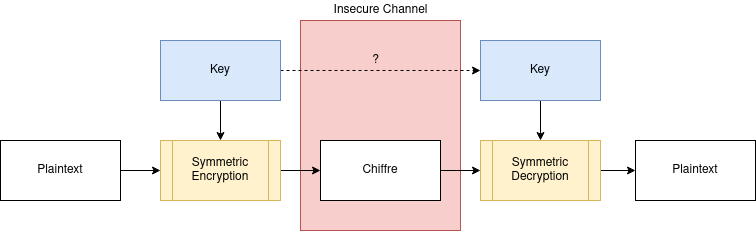
\includegraphics[width=0.8\textwidth]{background/symmetric_encryption}
  \caption[Symmetric encryption scheme]{Simple symmetric encryption scheme: Encryption and decryption algorithm use the same key.} \label{fig:symmetric-encryption}
\end{figure}

In the following, the symmetric decryption and encryption is expressed in a more formal way. The common key \textit{k} is used for encryption (\textit{Enc}) and decryption (\textit{Dec}), \textit{p} is the plaintext and \textit{c} is the ciphertext:

\begin{align*}
Enc(p, k) = c\\
Dec(c, k) = p
\end{align*}

\subsubsection{Asymmetric Cryptography}

In asymmetric cryptography each participating subject needs to generate a key pair, that consist of a private key and a public key. As mentioned above, the public key needs to be public (e.g. stored in a public database or a public key server). The private key is only known to the subject and needs to be kept secret.
\autoref{fig:asymmetric-encryption} shows an example for asymmetric encryption. Assume Alice wants to send encrypted data to Bob. Therefore, Bob created a key pair and published his public key. Alice requests Bobs public key (e.g. from a public database) and uses it to encrypt the data. Once Bob received the ciphertext, he uses his secret private key for decryption in order to retrieve the original  plaintext. In this work, the term \textit{public-key encryption} or \textit{public-key algorithm} is used as a synonym for asymmetric cryptography.

\begin{figure}[htpb]
  \centering
  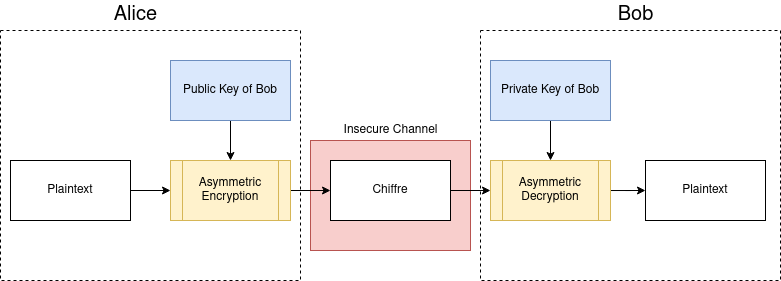
\includegraphics[width=0.8\textwidth]{background/asymmetric_encryption}
  \caption[Asymmetric encryption scheme]{Asymmetric encryption scheme: Encryption and decryption algorithm use different keys.} \label{fig:asymmetric-encryption}
\end{figure}
To formalize this procedure, again assume \textit{p} as plaintext and \textit{c} as ciphertext. The generated key pair of Bob consists of a private key for decryption ($d_{Bob}$) and a public key for encryption ($e_{Bob}$).

\begin{align*}
Enc(p, e_{Bob}) = c\\
Dec(c, d_{Bob}) = p
\end{align*}
\\
In contrast to the symmetric encryption, no secret key needs to be exchanged. However, the encryption and decryption of data using asymmetric encryption require intensive mathematical computations. Hence, the encryption of big sets of data using asymmetric encryption is not efficient.
One the other hand, symmetric encryption algorithms are usually based on simple operations, such as bit shifting or XOR. This can be implemented efficiently in software and hardware. Thus, the practical relevance of symmetric encryption is enormous~\parencite{ITSicherheit}.
\\
As stated above, securely exchanged keys are a precondition for the use of efficient symmetric encryption schemes. In order to exchange arbitrary keys securely, different key exchange protocols are available.

\section{Key Exchange}
\subsection{Diffie-Hellman Key-Exchange}

The Diffie-Hellman key exchange was introduced by Whitfield Diffie and Martin Hellman in 1976 ~\parencite{diffie1976new}. The resulting shared key of the protocol is calculated decentralized and is never transported over an insecure channel.

\subsubsection{Protocol}
The classical Diffie-Hellman key exchange assumes, that Alice and Bobs want to create a shared secret key. Therefore, they agree on a big prime $p$ and $g$, which is a primitive root modulo $p$\footnote{The primitive root modulo p is a generator element for the set S = $\{1, 2, ... , p-1\}$~\parencite{ITSicherheit}.}. Both, $p$ and $g$ are not secret and may be known to the public~\parencite{watjen2018kryptographie}.

\begin{enumerate}
\item Alice choses a random $a \in \{1, 2, ... , p-2\}$ as private key. 
\item Alice calculates the public key $A = g^a mod p$.
\item Bob choses a random $b \in \{1, 2, ... , p-2\}$ as private key. 
\item Bob calculates the public key $B = g^b mod p$.
\item Alice and Bob exchange their public keys $A$ and $B$.
\item Alice calculates: 
\begin{equation}
\begin{split}
k_{AB} & = B^a mod p \\
 & = (g^b mod p)^a mod p \\
 & = g^{a b} mod p
\end{split}
\end{equation}
\item Bob calculates: 
\begin{equation}
\begin{split}
k_{AB} & = A^b mod p \\
 & = (g^a mod p)^b mod p \\
 & = g^{b a} mod p \\
 & = g^{a b} mod p
\end{split}
\end{equation}
\item Alice and Bob created the shared secret $k_{AB}$. Note that only the public keys of Alice and Bob were send over an insecure channel. The generated secret was calculated decentralized by Alice and Bob.
\end{enumerate}
This procedure also can be illustrated in the following diagram, which emphasizes the commutative properties of the protocol. It does not matter if first apply $x \to x^a$ or $x \to x^b$ to the starting point $g$. The result is the same, since $g^{ab} = g^{ba}$.

\begin{figure}[htpb]
  \centering
  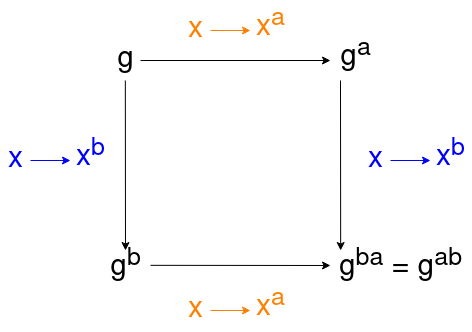
\includegraphics[width=0.5\textwidth]{background/diffie_hellman}
  \caption[Diffie Hellman diagram]{Diffie Hellman diagram, both paths lead to the same result.}
  \label{fig:diffie_hellman}
\end{figure}

\subsubsection{Security}
If an attacker wants to compute $k_{AB}$, it needs to compute the private keys $A$ and $B$ of Alice and Bob. Since only the public keys are exchanged, the attacker needs to compute:
\begin{equation*}
\begin{split}
b &= log_g\:B\:mod\;p\\ 
a &= log_g\:A\:mod\;p
\end{split}
\end{equation*}
\\
Hence, the security of the classical Diffie-Hellman key exchange is based on the discrete logarithm problem (see \ref{discrete_log_problem}). When using ephemeral key pairs, the Diffie-Hellman key exchange may be used as efficient perfect forward secrecy (PFS) protocol~\parencite{ITSicherheit}.
\\
In modern cryptography elliptic curves are often used to increase the security of the Diffie-Hellman key exchange (ECDH). The participants have to agree on an elliptic curve and and point $P$ on the elliptic curve. The computations to generate the shared secret $k_{AB}$ follow the same principles, but obviously they are adopted to work on elliptic curves. The advantage of ECDH is the increased security strength while using the same key length than the classical Diffie-Hellman protocol~\parencite{ITSicherheit}.
\\
Note that the introduced protocol does not authorize the participating subjects and does not guarantee integrity. Thus, this simple protocol may be exploited by a Man-In-The-Middle attack. A more advanced protocol using certificates and signed messaged could be implemented, to guarantee authentication and integrity~\parencite{ITSicherheit}.

\subsection{Key Encapsulation}

Key encapsulation methods (KEM) transmit a previously generated symmetric key. KEMs usually use asymmetric key pairs in order to encrypt the generated symmetric key. In the following the concept is shown by the RSA based PKCS \#1 v1.5 algorithm, which uses RSA key pairs to transmit a shared secret from Alice to Bob \parencite{rsakem}:

\begin{enumerate}
\item Bob generates a RSA key pair with the public key $e_{Bob}$ and the private key $d_{Bob}$ and transmits the public key to Alice.
\item Alice generates a random secret key $k_{AB}$:
\begin{equation*}
k_{AB} = random()
\end{equation*}
\item Alice maps this secret to an integer $m$, using a well-defined mapping function $h$:
\begin{equation*}
m = h(k_{AB})
\end{equation*}
\item Alice encrypts $m$ with Bobs public key using the RSA encryption algorithm and transmits $c$ to Bob.
\begin{equation*}
c = RSA_{enc}(m, e_{Bob})
\end{equation*}
\item Bob decrypts the received ciphertext $s$ to obtain the integer $m$:
\begin{equation*}
m = RSA_{dec}(c, d_{Bob})
\end{equation*}
\item Finally bob uses the inverse mapping function $h^{-1}$ to retrieve the shared secret:
\begin{equation*}
k_{AB} = h^{-1}(m1)
\end{equation*}

\end{enumerate}

\subsection{Differences}
TODO: differences betweent kem and kex (decentralized, pfs?), discrete log vs factorization

\section{Post-Quantum Cryptography}

In the following a \textit{classical computer} refers to a non-quantum computer, which can be simulated by a deterministic Turing machine. In contrast to \textit{classical computer} the term \textit{quantum computer} describes a machine, which uses quantum mechanical phenomena to perform computations. It is important to note, that quantum computers can simulate classical computers. In addition, classical computer are able to simulate quantum computers with exponential time overhead. Thus, classical and quantum computations can calculate the same class of functions. However, quantum computers enable operations, that allow much faster computation~\parencite{nielsen2002quantum}.\\
In the past, scientists queried, if large-scale quantum computer are a physical possibility. It was stated, that the underlying quantum states are too fragile and hard to control. \parencite{chen2016report} Today, quantum error correction codes are known, which put a large-scale quantum computers within the realms of possibility~\parencite{lidar2013quantum}. However, it is still a big engineering challenge from a laboratory approach to a general-purpose quantum computer, which involves thousands or millions of physical qubits~\parencite{chen2016report}.
\\\\
The security of modern asymmetric cryptographic primitives is usually based on difficult number theoretic problems, e.g. the discrete logarithm problem (DH, ECDH) or the factorization problem (RSA)~\parencite{chen2016report}. These problems are theoretically solvable, but the computation of a result on classical computer claims an impractical amount of resources. In 2019, scientists solved the factorization problem for a 240 digit integer in about 900 core-years on a classical computer (one core year means running a CPU for a full year)~\parencite{boudot2795}. In the following the discrete logarithm problem and the factorization problem are described.

\subsubsection{Discrete Logarithm Problem} \label{discrete_log_problem}
The discrete logarithm problem is the following challenge \parencite{beutelspacher2010diskrete}: Given a prim $p$ and two integers $g$ and $y$. Find an integer $x$, such that
\begin{equation*}
\begin{split}
&y = g^x mod p \\
\iff &x = log_g\;y\:mod p
\end{split}
\end{equation*}
Until today, it is not known if a classical computer is able to compute the general discrete logarithm problem in polynomial time. Thus, the discrete logarithm problem is considered to be difficult so solve for classical computers~\parencite{beutelspacher2010diskrete}. This assumption makes the discrete logarithm problem an attractive basis for DSA, ElGamal, the classical Diffie-Hellman protocol, and for the elliptic curve Diffie-Hellman (ECDH).

\subsubsection{Factorization Problem}

Given two large primes p and q, it is easy to compute the the product of them:
\begin{equation*}
n = p \star q
\end{equation*}
For a given $n$, however, it is difficult to find the prime factors $p$ and $q$. The computation of the prime factorization for a given integer $n$ is called the factorization problem~\parencite{ITSicherheit}. For large numbers n no efficient algorithm for classical computers is known to solve this challenge~\parencite{ITSicherheit}. The most famous cryptographic protocol, which builds upon the hardness of the factorization problem is RSA.

\subsection{Impact of Quantum Computers on Cryptography}

As stated above, quantum computers enable new operations which speed up certain algorithms. Two quantum algorithms which have enormous consequences on modern cryptography are \textit{Shor's algorithm} and \textit{Grover's algorithm}~\parencite{nielsen2002quantum}.

\subsubsection{Shor's Algorithm}
Peter Shor published \textit{"Algorithms for quantum computation: discrete logarithms and factoring"} in 1994 \parencite{shor1994algorithms}, where he demonstrated that the factorization problem and the discrete logarithm problem can be solved in polynomial time on quantum computers. Both problems are the basis of many public-key systems (RSA, DH, ECDH, ...), which are used intensively in modern communication systems. Hence, a quantum computer running \textit{Shor's algorithm} would qualify the assumption of most asymmetric encryption schemes and thus break their security.


\subsubsection{Grover's Algorithm}
The second algorithm having impact on computer security was published by Lov Grover in 1996 (\textit{"A fast quantum mechanical algorithm for database search"}, \parencite{grover1996fast}) - namely \textit{Grover's algorithm}. The algorithms solves the problem of finding an element $y$ in a set $s$ (e.g. a database) where $|s| = N$. On a classical computer an algorithm solving the problem runs in $\mathcal{O}(N)$, however \textit{Grover's algorithm} has complexity $\mathcal{O}(\sqrt{N})$~\parencite{nielsen2002quantum}.\\
In contrast to public-key systems, which relay on hard mathematical problems, symmetric encryption schemes relay on the secrecy of a randomly generated key. 
Thus, to break symmetric encryption one need to perform a brute-force attack on the symmetric key. Using \textit{Grover's algorithm} offers a square root speed up on classical brute force attacks~\parencite{mavroeidis2018impact}. Assume a randomly generated $n$-bit key. A classical brute force algorithm lies in $\mathcal{O}(2^n)$, which is considered to be safe for a big $n$ (e.g. $n$=128). \textit{Grover's algorithm} speeds up this attack to $\mathcal{O}(\sqrt{2^n})$ = $\mathcal{O}(2^{n/2})$~\parencite{mavroeidis2018impact}. However, the complexity is still exponential and with a growing key size $n$ the security can be further increased. Thus, \textit{Grover's algorithm} forces symmetric encryption schemes to increase their used key size in order to stay secure.
\\\\
To sum up, quantum computers make use of quantum mechanical phenomena in order to solve mathematical problems, which are assumed to be difficult for modern computers. As a result large-scale quantum computers might break many algorithms of modern asymmetric cryptography and enforce increased key sizes for symmetric encryption schemes. The following table form the NIST \textit{"Report on Post-Quantum Cryptography"} \parencite{chen2016report} shows the impact of quantum computers on modern encryption schemes:

\begin{table}[htpb]
  \centering
  \begin{tabular}{|K{3cm}|K{3cm}|K{4cm}|K{4cm}|}
	\hline
    \rowcolor{lightgray!50}
      \textbf{Cryptographic} \textbf{algorithm} & \textbf{Type} & \textbf{Purpose} & \textbf{Impact from} \textbf{ quantum computer} \\
	\hline
      AES & Symmetric key & Encryption & Larger key sizes needed \\
    \hline
      SHA & --- & Hash functions & Larger output needed \\
    \hline
      RSA & Public key & Signatures, key establishment & No longer secure \\
	\hline      
      DSA & Publiy key & Signatures, key exchange & No longer secure \\
    \hline
      ECDH, ECDSA & Public key & Signatures, key exchange & No longer secure \\
    \hline
  \end{tabular}
  \caption[Impact of quantum computers on modern encryption schemes]{Impact of quantum computers on modern encryption schemes}\label{tab:impact}
\end{table}

In contrast to this development in modern cryptography NIST states~\parencite{chen2016report}:
\begin{quote}
\textit{"In the last three decades, public key cryptography has become an indispensable component of our global communication digital infrastructure. These networks support a plethora of applications that are important to our economy, our security, and our way of life, such as mobile phones, internet commerce, social networks, and cloud computing. In such a connected world, the ability of individuals, businesses and governments to communicate securely is of the utmost importance."}
\end{quote}
This statement emphasizes the urgency and need of new asymmetric encryption schemes. As a consequence, NIST initiated a process to standardize quantum-secure public-key algorithms. In literature, this is called \textit{post-quantum cryptography}, since the objectives of the submitted procedures is to stay secure against a large-scale quantum computer. In July 2020, Round 3 of the standardization process was announced. Different approaches for quantum-resistant algorithms have been proposed. In this work, the focus is on isogeny-based cryptography (section \ref{sec:isogeny-based_crypto}). Other classes of post-quantum cryptography are described for completeness in the following section \ref{sec:classes_pqc}.

\subsection{Classes of Post-Quantum Cryptography} \label{sec:classes_pqc}

This section provides an overview about important post-quantum cryptography classes: Lattice-based, multivariate and code-based cryptography as well as hash-based signatures are shortly presented. 

\subsubsection{Lattice-based Cryptography}
Lattice-based cryptography is - as the name suggests - based on the mathematical construct of lattices\footnote{A lattice $l$ is a subgroup of $\mathbb{R}^n$. In the context of cryptography usually integer lattices are considered: $l \subseteq \mathbb{Z}^n$ \parencite{chi2015lattice}.}. There are different computational optimization problems involving lattices, which are considered to be hard to solve even for quantum computers~\parencite{chi2015lattice}. In 1998, NTRU was published as the first public-key system based on lattices ~\parencite{hoffstein1998ntru}. Since then NTRU was continuously improved resulting in NTRUencrypt (public-key system) and NTRUsign (digital signing algorithm). Furthermore, a fully homomorphic encryption scheme based on lattices was published in 2009~\parencite{gentry2009fully}.\\
Lattice-based cryptography is characterized by simplicity and efficiency \parencite{chen2016report}. The security of existing implementations (NTRU or Ring-LWE) can be reduced to NP-hard problems. However, lattices encryption schemes have problems to prove security against known cryptoanalysis \parencite{chen2016report}.
\subsubsection{Multivariate Cryptography}
Multivariate cryptography are public key systems that are based on multivariate polynomials (e.g. $p(x,y)=x+2y$) over a finite field $\mathbb{F}$. Their security is based on the prove, that solving systems of multivariate polynomials are NP-hard~\parencite{hartmanis1982computers}. This makes multivariate public key systems attractive for post-quantum cryptography; especially their short signatures make them a candidate for quantum-secure digital signature algorithms~\parencite{ding2017current}, e.g. the Rainbow signature scheme~\parencite{ding2005rainbow}.
\subsubsection{Code-based Cryptography}
Code-based cryptographic primitives are build upon error-correcting codes. A public key system using error-correcting codes uses a public key to add errors to a given plaintext resulting in a ciphertext. Only the owner of the private key is able to correct there errors and to reconstruct the plaintext~\parencite{bernstein2017post}. McEliece, published in 1978, was the first of those systems and it has not been broken until today~\parencite{mceliece1978public}.
Beside asymmetric cryptography, code-based schemes have been proposed for digital signatures, random number generators and cryptographic hash functions~\parencite{bernstein2017post}.
\subsubsection{Hash-based Signatures}
Hash-based signatures describe the construction of digital signatures schemes based on hash functions. Thus, the security of theses primitives is based on the security of the underlying hash function and not on hard algorithmic problems~\parencite{bernstein2017post}. Since hash functions are widely deployed in modern computer systems, the security of hash-based signatures is well understood~\parencite{chen2016report}.\\
The initially developed One-Time Signatures have the downside, that a new public key pair is needed for each signature~\parencite{becker2008merkle}. In 1979, Merkle introduced the Merkle Signature Scheme (MSS), which uses one public key for multiple signatures~\parencite{merkle1979secrecy}. Further improvements of MSS introduced public keys, which can be used for $2^{80}$ signatures. However, this also leads to longer signature sizes~\parencite{becker2008merkle}.

\subsection{Isogeny-based Cryptography} \label{sec:isogeny-based_crypto}
Isogeny-based cryptography was proposed in 2011 as a new cryptographic system, that might resists quantum computing~\parencite{jao2011towards}. Beside the publication describing isogeny-based cryptgraphy, the authors also provided a reference implementaion of a public key system, which is called SIKE~\parencite{sike2020spec}. Isogeny-based cryptography benfits from small key sizes compared to other post-quantum cryptography classes, however, their performance is comparatively slow~\parencite{sike2020spec}. The security of these primitives is based on finding isogenies between supersingular elliptic curves.\\
In the following, the problem is roughly illustrated. It is not indented to precise the mathematics behind isogeny-based cryptography, since this is not the scope of this work. However, the reader might become a little understanding of the magic behind supersingular isogenies. Next, the central component of isogeny-based cryptography, namely the Supersingular Isogeny Diffie Hellman (SIDH), is described. Finally, details of the reference implementation SIKE will be given.

\subsubsection{Illustration of the Problem ~\parencite{urbanik2017friendly}~\parencite{costello2019supersingular}}
Isogeny-based cryptography works on supersingular elliptic curves. To be more precise, it is based on isogenies between supersingular elliptic curves.
\\
In the context of elliptic curves, one can calculate a quotient of an elliptic curve $E$ by a subgroup $S$. This essentially means to construct a new elliptic curve $E$\textbackslash $S$.
Beside this new curve, the procedure also yields a function $\phi_S: E \to E \backslash S$, which is called \textit{isogeny}. Carefully chosen elliptic curves E have a wide range of subgroups, which can be used to construct many isogenies.
\\
Supersingular elliptic curves are a special type of elliptic curves, which have properties that are useful for cryptography. Since supersingular elliptic curves can be seen as subset from ordinary elliptic curves, they can also be used to calculate isogenies between certain curves, as described above.
\\
The idea behind isogeny-based cryptography might be illustrated as followed:

\begin{enumerate}
\item Start with a known curve $E$ and build a isogeny to a arbitrary reachable curve $E_A$.
\item This yields the isogeny $\phi_A: E \to E_A$, which is used as private key.
\item The curve $E_A$ is used as part of the public key.
\end{enumerate}
As usually in asymmetric cryptography, the hard mathematical problem is the calculation of the private key while knowing the public key. To be more precise: Find the isogeny $\phi_A: E \to E_A$ while knowing curves $E$ and $E_A$ is considered to be a quantum-resistant challenge. In literature, this is formally defined as \textit{SIDH problem}~\parencite{sike2020spec}. 
\\
This key pair, however, is not used to decrypt or encrypt data. In fact, the procedure is very similar to the previously introduced Diffie-Hellman key exchange, where the key pair is used to establish a shared secret between two communication partners.
In its core, isogney-based cryptography creates a shared secret via a Diffie-Hellman like procedure. This is called \textit{Supersingular Isogeny Diffe Hellman (SIDH)}.

\subsubsection{Supersingular Isogeny Diffie Hellman (SIDH)}

Recall the Diffie Hellman diagram in  \autoref{fig:diffie_hellman}, where the commutative property of the protocol was shown. The same diagram can be drawn for the Diffie Hellman on supersingular isogenies, see \autoref{fig:sidh}. 
\begin{figure}[H]
  \centering
  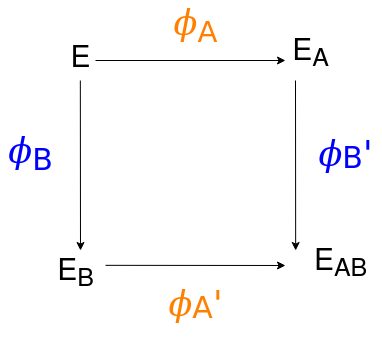
\includegraphics[width=0.5\textwidth]{background/sidh}
  \caption[Supersingular Isogeny Diffie Hellman diagram]{Supersingular Isogeny Diffie Hellman procedure, both paths lead to the same result. Note, the different isogenies $\phi_{A}'$ and $\phi_{B}'$, that are applied in each second step of the diagram. The reason for this lies in the mathematics of supersingular isogenies: $\phi_{A} \phi_{B} \neq \phi_{B} \phi_{A}$. In order to construct $\phi_{X}'$ or $\phi_{B}'$, the public key of each communication partner provides additional information beside the curve $E_A$ or $E_B$.~\parencite{costello2016gentle}}
  \label{fig:sidh}
\end{figure}
In the previous section the underlying mathematical idea was illustrated. The described key generation can be extended to a key exchange primitive, which has strong similarity to the classical Diffie-Hellman key exchange. Starting point of SIDH is a known supersingular elliptic curve E. 

\begin{enumerate}
\item Alice creates an isogeny $\phi_A$ (private key), which leads to curve $E_A$ (part of the public key).
\item Bob creates an isogeny $\phi_B$ (private key), which leads to curve $E_B$ (part of the public key).
\item Alice and Bob exchange their public keys.
\item Bob computes $\phi_B'$ (using additional information from the public key of Alice) and applies $\phi_B'$ to the received $E_A$. This results in $E_{AB}$
\item Alice computes $\phi_A'$ (using additional information from the public key of Bob) and applies $\phi_A'$ to the received $E_B$. This results in $E_{AB}$
\item Alice and Bob now share the  common secret $E_{AB}$.
\end{enumerate}

\subsubsection{Implemenation Details}

The reference implementation of SIKE \parencite{sike2020spec} provides two fundamental functions: \textit{isogen} and \textit{isoex}. Both are used, to implement the previously introduced Supersingular Isogeny Diffie-Hellman (SIDH) algorithm. Note, that the secret key \textit{sk} is represented as a random integer.
\\

\begin{table}[H]
  \centering
  \begin{tabular}{|K{3cm}|K{3cm}|K{4cm}|}
	\hline
    \rowcolor{lightgray!50}
      \textbf{Function} & \textbf{Input} & \textbf{Output} \\
	\hline
      \textit{isogen} & secret key \textit{sk} & public key \textit{pk} \\
     \hline
      \textit{isoex} & secret key \textit{sk}, public key \textit{pk} & shared secret \textit{sec}\\
     \hline
  \end{tabular}
   \caption[Core functions of the SIKE reference implementation]{Core functions of the SIKE reference implementation.}\label{tab:sike_core_functions}
\end{table}

The function \textit{isogen} takes a secret key (random integer) as input an generates the public key. The shared secret is generated by \textit{isoex}, which takes the own secret key and the foreign public key as input. The key exchange procedure with respect to \textit{isogen} and \textit{isoex} works as followed:


\begin{figure}[H]
  \centering
  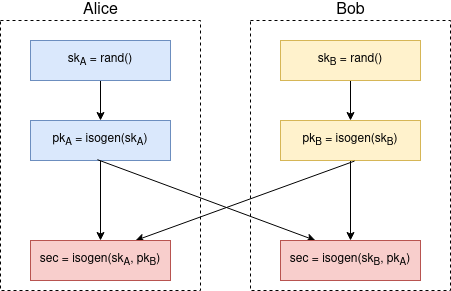
\includegraphics[width=0.6\textwidth]{background/sike_sidh}
  \caption[SIDH based on \textit{isogen} and \textit{isoex}]{SIDH based on \textit{isogen} and \textit{isoex}: After generating a random secret key \textit{sk}, each party computes its public key \textit{pk}. After the exchange of public keys, each party finally calculates the shared secret \textit{sec}.} \label{fig:sike-sidh}
\end{figure}
Beside this key exchange algorithm, SIKE provides a complete asymmetric encryption scheme and a key encpsulation mechansim (KEM)~\parencite{sike2020spec}. 
Both of these schemes build upon the here described SIKE core functions \textit{isogen} and \textit{isoex}.

\begin{figure}[H]
  \centering
  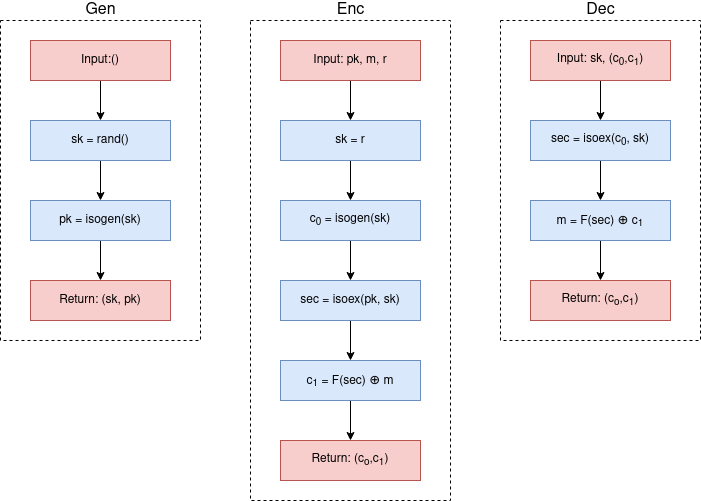
\includegraphics[width=0.8\textwidth]{background/sike_asym}
  \caption[SIKE public key encryption]
  {The SIKE public key encryption system consists of three algorithms: 
  \\
  1. \textit{Gen} generates a key pair \textit{(sk, pk)}.
  \\
  2. \textit{Enc} encrypts a given plaintext $m$ using a foreign public key \textit{pk} and the own secret key \textit{r}.
  \\
  3. \textit{Dec} decodes a given cipthertext using the own secret key \textit{sk}.
  \\ Note, that the function $F$ used in \textit{Enc} and \textit{Dec} is a key derivation function.} \label{fig:sike-sidh}
\end{figure}

\begin{figure}[H]
  \centering
  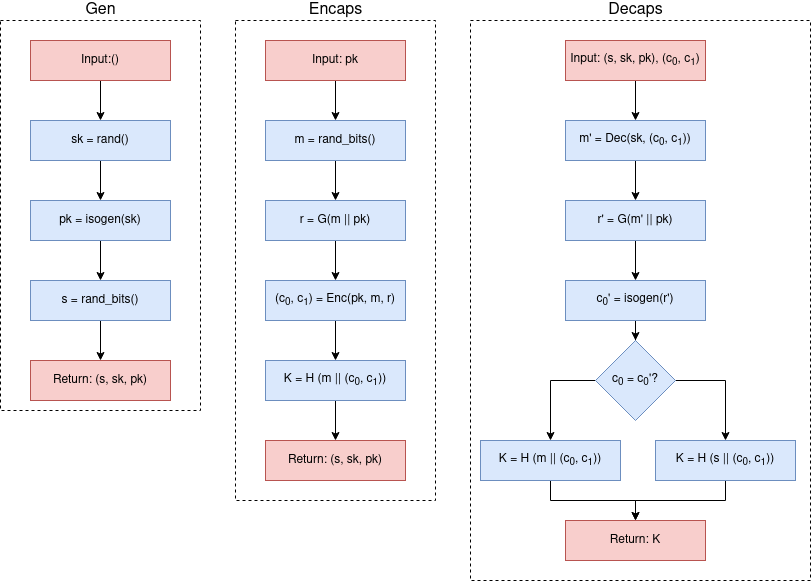
\includegraphics[width=0.8\textwidth]{background/sike_kem}
  \caption[SIKE public key encryption]
  {The SIKE key exchange mechanism consists of three algorithms: 
  \\
  1. \textit{Gen} TODO
  \\
  2. \textit{Encaps} TODO
  \\
  3. \textit{Decaps} TODO
  } \label{fig:sike-sidh}
\end{figure}

\subsubsection{Security considerations}
The security of SIKE is based on the hardness of the \textit{SIDH problem}: Given two supersingular elliptic curves $E$ and $E'$, find an isogeny between them~\parencite{sike2020spec}. 
\\
The SIKE reference implementation proposes different parameter sets, each supposing to ensure a NIST defined security level. These NIST defined security levels are:
\begin{enumerate}
	\item Any attack breaking this security level must require resources comparable to perform a key search on a 128-bit key (e.g. AES128).
	\item Any attack breaking this security level must require resources comparable to perform a collision search search on a 256-bit hash function (e.g. SHA256).
	\item Any attack breaking this security level must require resources comparable to perform a key search on a 192-bit key (e.g. AES192).
	\item Any attack breaking this security level must require resources comparable to perform a collision search search on a 384-bit hash function (e.g. SHA384).
	\item Any attack breaking this security level must require resources comparable to perform a key search on a 256-bit key (e.g. AES256).
\end{enumerate}
The proposed parameter sets of SIKE are named after the bit length of the underlying primes:

\begin{itemize}
	\item \texttt{SIKEp434} supposed to satisfy NIST securiy level 1 (AES128)
	\item \texttt{SIKEp503} supposed to satisfy NIST securiy level 2 (SHA256)
	\item \texttt{SIKEp610} supposed to satisfy NIST securiy level 3 (AES192)
	\item \texttt{SIKEp751} supposed to satisfy NIST securiy level 5 (AES256)
\end{itemize}
Current research provides confidence, that the SIKE parameter sets satisfy the defined security levels even under the assumption of currently known algorithms~\parencite{jaques2019quantum}. Therefore, the authors consider three algorithms to solve the \textit{SIDH problem}: \textit{Tani's quantum claw finding algorithm}~\parencite{tani2009claw}, \textit{Grover's algorithm}~\parencite{grover1996fast} and a \textit{parallel collision-finding algorithm}~\parencite{van1999parallel}.
\\\\
Ephemeral SIDH keys are predestined to implement quantum-secure perfect forward secrecy protocols (PFS)~\parencite{longa2018note}. PFS ensures, that a compromised long-term key does not reveal past or future keys of the protocol.
\\\\
Side-channel attacks against isogeny-basd cryptography might 1) reveal parts of the secret private key or 2) reveal parts of the public key computation. To protect against power-analysis side-channel attacks it is recommend to prefer constant-time implementations~\parencite{sike2020spec}. The authors state, however, that an attacker has \textit{"access to a wide range of power, timing, fault and various other side-channels"}. Thus, preventing isogeny-based cryptography from all side-channel attacks seems to be nearly impossible.
